
\documentclass[a4paper,11pt]{article}
\usepackage[a4paper, margin=8em]{geometry}

% usa i pacchetti per la scrittura in italiano
\usepackage[french,italian]{babel}
\usepackage[T1]{fontenc}
\usepackage[utf8]{inputenc}
\frenchspacing 

% usa i pacchetti per la formattazione matematica
\usepackage{amsmath, amssymb, amsthm, amsfonts}

% usa altri pacchetti
\usepackage{gensymb}
\usepackage{hyperref}
\usepackage{standalone}

\usepackage{colortbl}

\usepackage{xstring}
\usepackage{karnaugh-map}

% imposta il titolo
\title{Specification and Simulation of Digital Systems notes}
\author{Luca Seggiani}
\date{2026}

% imposta lo stile
% usa helvetica
\usepackage[scaled]{helvet}
% usa palatino
\usepackage{palatino}
% usa un font monospazio guardabile
\usepackage{lmodern}

\renewcommand{\rmdefault}{ppl}
\renewcommand{\sfdefault}{phv}
\renewcommand{\ttdefault}{lmtt}

% circuiti
\usepackage{circuitikz}
\usetikzlibrary{babel}

% testo cerchiato
\newcommand*\circled[1]{\tikz[baseline=(char.base)]{
            \node[shape=circle,draw,inner sep=2pt] (char) {#1};}}

% disponi il titolo
\makeatletter
\renewcommand{\maketitle} {
	\begin{center} 
		\begin{minipage}[t]{.8\textwidth}
			\textsf{\huge\bfseries \@title} 
		\end{minipage}%
		\begin{minipage}[t]{.2\textwidth}
			\raggedleft \vspace{-1.65em}
			\textsf{\small \@author} \vfill
			\textsf{\small \@date}
		\end{minipage}
		\par
	\end{center}

	\thispagestyle{empty}
	\pagestyle{fancy}
}
\makeatother

% disponi teoremi
\usepackage{tcolorbox}
\newtcolorbox[auto counter, number within=section]{theorem}[2][]{%
	colback=blue!10, 
	colframe=blue!40!black, 
	sharp corners=northwest,
	fonttitle=\sffamily\bfseries, 
	title=Theorem~\thetcbcounter: #2, 
	#1
}

% disponi definizioni
\newtcolorbox[auto counter, number within=section]{definition}[2][]{%
	colback=red!10,
	colframe=red!40!black,
	sharp corners=northwest,
	fonttitle=\sffamily\bfseries,
	title=Definition~\thetcbcounter: #2,
	#1
}

% disponi codice
\usepackage{listings}
\usepackage[table]{xcolor}

\definecolor{codegreen}{rgb}{0,0.6,0}
\definecolor{codegray}{rgb}{0.5,0.5,0.5}
\definecolor{codepurple}{rgb}{0.58,0,0.82}
\definecolor{backcolour}{rgb}{0.95,0.95,0.92}

\lstdefinestyle{codestyle}{
		backgroundcolor=\color{black!5}, 
		commentstyle=\color{codegreen},
		keywordstyle=\bfseries\color{magenta},
		numberstyle=\sffamily\tiny\color{black!60},
		stringstyle=\color{green!50!black},
		basicstyle=\ttfamily\footnotesize,
		breakatwhitespace=false,         
		breaklines=true,                 
		captionpos=b,                    
		keepspaces=true,                 
		numbers=left,                    
		numbersep=5pt,                  
		showspaces=false,                
		showstringspaces=false,
		showtabs=false,                  
		tabsize=2
}

\lstdefinestyle{shellstyle}{
		backgroundcolor=\color{black!5}, 
		basicstyle=\ttfamily\footnotesize\color{black}, 
		commentstyle=\color{black}, 
		keywordstyle=\color{black},
		numberstyle=\color{black!5},
		stringstyle=\color{black}, 
		showspaces=false,
		showstringspaces=false, 
		showtabs=false, 
		tabsize=2, 
		numbers=none, 
		breaklines=true
}

\lstdefinelanguage{x86}{ 
  keywords={AAA, AAD, AAM, AAS, ADC, ADCB, ADCW, ADCL, ADD, ADDB, ADDW, ADDL, AND, ANDB, ANDW, ANDL,
        ARPL, BOUND, BSF, BSFL, BSFW, BSR, BSRL, BSRW, BSWAP, BT, BTC, BTCB, BTCW, BTCL, BTR, 
        BTRB, BTRW, BTRL, BTS, BTSB, BTSW, BTSL, CALL, CBW, CDQ, CLC, CLD, CLI, CLTS, CMC, CMP,
        CMPB, CMPW, CMPL, CMPS, CMPSB, CMPSD, CMPSW, CMPXCHG, CMPXCHGB, CMPXCHGW, CMPXCHGL,
        CMPXCHG8B, CPUID, CWDE, DAA, DAS, DEC, DECB, DECW, DECL, DIV, DIVB, DIVW, DIVL, ENTER,
        HLT, IDIV, IDIVB, IDIVW, IDIVL, IMUL, IMULB, IMULW, IMULL, IN, INB, INW, INL, INC, INCB,
        INCW, INCL, INS, INSB, INSD, INSW, INT, INT3, INTO, INVD, INVLPG, IRET, IRETD, JA, JAE,
        JB, JBE, JC, JCXZ, JE, JECXZ, JG, JGE, JL, JLE, JMP, JNA, JNAE, JNB, JNBE, JNC, JNE, JNG,
        JNGE, JNL, JNLE, JNO, JNP, JNS, JNZ, JO, JP, JPE, JPO, JS, JZ, LAHF, LAR, LCALL, LDS,
        LEA, LEAVE, LES, LFS, LGDT, LGS, LIDT, LMSW, LOCK, LODSB, LODSD, LODSW, LOOP, LOOPE,
        LOOPNE, LSL, LSS, LTR, MOV, MOVB, MOVW, MOVL, MOVSB, MOVSD, MOVSW, MOVSX, MOVSXB,
        MOVSXW, MOVSXL, MOVZX, MOVZXB, MOVZXW, MOVZXL, MUL, MULB, MULW, MULL, NEG, NEGB, NEGW,
        NEGL, NOP, NOT, NOTB, NOTW, NOTL, OR, ORB, ORW, ORL, OUT, OUTB, OUTW, OUTL, OUTSB, OUTSD,
        OUTSW, POP, POPL, POPW, POPB, POPA, POPAD, POPF, POPFD, PUSH, PUSHL, PUSHW, PUSHB, PUSHA, 
        RCLL, RCR, RCRB, RCRW, RCRL, RDMSR, RDPMC, RDTSC, REP, REPE, REPNE, RET, ROL, ROLB, ROLW,
        ROLL, ROR, RORB, RORW, RORL, SAHF, SAL, SALB, SALW, SALL, SAR, SARB, SARW, SARL, SBB,
        SBBB, SBBW, SBBL, SCASB, SCASD, SCASW, SETA, SETAE, SETB, SETBE, SETC, SETE, SETG, SETGE,
        SETL, SETLE, SETNA, SETNAE, SETNB, SETNBE, SETNC, SETNE, SETNG, SETNGE, SETNL, SETNLE,
        SETNO, SETNP, SETNS, SETNZ, SETO, SETP, SETPE, SETPO, SETS, SETZ, SGDT, SHL, SHLB, SHLW,
        SHLL, SHLD, SHR, SHRB, SHRW, SHRL, SHRD, SIDT, SLDT, SMSW, STC, STD, STI, STOSB, STOSD,
        STOSW, STR, SUB, SUBB, SUBW, SUBL, TEST, TESTB, TESTW, TESTL, VERR, VERW, WAIT, WBINVD,
        XADD, XADDB, XADDW, XADDL, XCHG, XCHGB, XCHGW, XCHGL, XLAT, XLATB, XOR, XORB, XORW, XORL},
  keywordstyle=\color{blue}\bfseries,
  ndkeywordstyle=\color{darkgray}\bfseries,
  identifierstyle=\color{black},
  sensitive=false,
  comment=[l]{\#},
  morecomment=[s]{/*}{*/},
  commentstyle=\color{purple}\ttfamily,
  stringstyle=\color{red}\ttfamily,
  morestring=[b]',
  morestring=[b]"
}

\lstdefinelanguage{riscv}{
  keywords={
    LUI, AUIPC,
    JAL, JALR,
    BEQ, BNE, BLT, BGE, BLTU, BGEU,
    LB, LH, LW, LBU, LHU, LD,
    SB, SH, SW, SD,
    ADDI, SLTI, SLTIU, XORI, ORI, ANDI,
    SLLI, SRLI, SRAI,
    ADD, SUB, SLL, SLT, SLTU, XOR, SRL, SRA, OR, AND,
    ADDIW, SLLIW, SRLIW, SRAIW,
    ADDW, SUBW, SLLW, SRLW, SRAW,
    MUL, MULH, MULHSU, MULHU, DIV, DIVU, REM, REMU,
    MULW, DIVW, DIVUW, REMW, REMUW,
    LR.W, SC.W, AMOSWAP.W, AMOADD.W, AMOXOR.W,
    AMOAND.W, AMOOR.W, AMOMIN.W, AMOMAX.W,
    AMOMINU.W, AMOMAXU.W,
    LR.D, SC.D, AMOSWAP.D, AMOADD.D, AMOXOR.D,
    AMOAND.D, AMOOR.D, AMOMIN.D, AMOMAX.D,
    AMOMINU.D, AMOMAXU.D,
    FLW, FSW,
    FMADD.S, FMSUB.S, FNMSUB.S, FNMADD.S,
    FADD.S, FSUB.S, FMUL.S, FDIV.S, FSQRT.S,
    FSGNJ.S, FSGNJN.S, FSGNJX.S,
    FMIN.S, FMAX.S,
    FCVT.W.S, FCVT.WU.S, FCVT.S.W, FCVT.S.WU,
    FMV.X.W, FMV.W.X,
    FEQ.S, FLT.S, FLE.S,
    FLD, FSD,
    FMADD.D, FMSUB.D, FNMSUB.D, FNMADD.D,
    FADD.D, FSUB.D, FMUL.D, FDIV.D, FSQRT.D,
    FSGNJ.D, FSGNJN.D, FSGNJX.D,
    FMIN.D, FMAX.D,
    FCVT.W.D, FCVT.WU.D, FCVT.D.W, FCVT.D.WU,
    FCVT.S.D, FCVT.D.S,
    FMV.X.D, FMV.D.X,
    FEQ.D, FLT.D, FLE.D,
    CSRRW, CSRRS, CSRRC,
    CSRRWI, CSRRSI, CSRRCI,
    FENCE.I,
    FENCE,
    ECALL, EBREAK,
    MRET, SRET, URET,
    WFI,
    SFENCE.VMA,
    NOP, LI, LA, MV,
    NOT, NEG, NEGW,
    SEQZ, SNEZ, SLTZ, SGTZ,
    BEQZ, BNEZ, BLEZ, BGEZ, BLTZ, BGTZ,
    BGT, BLE, BGTU, BLEU,
    J, JR, RET,
    CALL, TAIL,
    RDINSTRET, RDCYCLE, RDTIME,
    CSRR, CSRW, CSRS, CSRC,
    CSRWI, CSRSI, CSRCI
  },
  keywordstyle=\color{blue}\bfseries,
  ndkeywordstyle=\color{darkgray}\bfseries,
  identifierstyle=\color{black},
  sensitive=false,
  comment=[l]{\#},
  morecomment=[s]{/*}{*/},
  commentstyle=\color{purple}\ttfamily,
  stringstyle=\color{red}\ttfamily,
  morestring=[b]',
  morestring=[b]"
}

\lstdefinelanguage{arm}{
  keywords={
    ADC, ADD, AND, BIC, CMN, CMP, EOR, MOV, MVN,
    RSB, RSC, SBC, SUB, TST, TEQ,
    MLA, MLS, MUL, SMLAL, SMULL, UMLAL, UMULL,
    QADD, QSUB, QDADD, QDSUB,
    QADD16, QADD8, QASX, QSAX,
    QSUB16, QSUB8, QSAX, QSUBADDX,
    ASR, LSL, LSR, ROR, RRX,
    B, BL, BX, BLX,
    BXJ,
    BEQ, BNE, BCS, BHS, BCC, BLO,
    BMI, BPL, BVS, BVC,
    BHI, BLS, BGE, BLT, BGT, BLE,
    BAL,
    LDR, LDRB, LDRH, LDRSB, LDRSH,
    LDRD, LDM, LDMIA, LDMIB, LDMDA, LDMDB,
    LDRT, LDRBT, LDRHT, LDRSBT, LDRSHT,
    STR, STRB, STRH, STRD,
    STM, STMIA, STMIB, STMDA, STMDB,
    STRT, STRBT, STRHT,
    PUSH, POP,
    SWP, SWPB,
    REV, REV16, REVSH,
    BFC, BFI, BFXIL, SBFX, UBFX,
    CLZ,
    LDREX, LDREXB, LDREXH, LDREXD,
    STREX, STREXB, STREXH, STREXD,
    DMB, DSB, ISB,
    MCR, MCRR, MRC, MRRC,
    MRS, MSR,
    CPS, SETEND, SVC, BKPT,
    CLREX, WFE, WFI, SEV,
    YIELD, NOP,
    VLDR, VSTR,
    VMOV, VABS, VNEG,
    VADD, VSUB, VMUL, VDIV,
    VMLA, VMLS, VNMLA, VNMLS, VNMUL,
    VMAX, VMIN,
    VSQRT,
    VCMP, VCMPE,
    VCVT,
    VCLZ, VCLS,
    VAND, VORR, VEOR, VBIC, VMVN,
    VLD1, VLD2, VLD3, VLD4,
    VST1, VST2, VST3, VST4,
    ADR, ADCS, ADDS, SUBS, MOVS, ANDS, ORRS, EORS
  },
  keywordstyle=\color{blue}\bfseries,
  ndkeywordstyle=\color{darkgray}\bfseries,
  identifierstyle=\color{black},
  sensitive=false,
  comment=[l]{@},
  morecomment=[l]{;},
  morecomment=[s]{/*}{*/},
  commentstyle=\color{purple}\ttfamily,
  stringstyle=\color{red}\ttfamily,
  morestring=[b]',
  morestring=[b]"
}

\lstset{style=codestyle, language=C}

% disponi sezioni
\usepackage{titlesec}

\titleformat{\section}
	{\sffamily\Large\bfseries} 
	{\thesection}{1em}{} 
\titleformat{\subsection}
	{\sffamily\large\bfseries}   
	{\thesubsection}{1em}{} 
\titleformat{\subsubsection}
	{\sffamily\normalsize\bfseries} 
	{\thesubsubsection}{1em}{}

% tikz
\usepackage{tikz}

% float
\usepackage{float}

% grafici
\usepackage{pgfplots}
\pgfplotsset{width=10cm,compat=1.9}

% disponi alberi
\usepackage{forest}

\forestset{
	rectstyle/.style={
		for tree={rectangle,draw,font=\large\sffamily}
	},
	roundstyle/.style={
		for tree={circle,draw,font=\large}
	}
}

% disponi algoritmi
\usepackage{algorithm}
\usepackage{algorithmic}
\makeatletter
\renewcommand{\ALG@name}{Algorithm}
\makeatother

% disponi numeri di pagina
\usepackage{fancyhdr}
\fancyhf{} 
\fancyfoot[L]{\sffamily{\thepage}}

\makeatletter
\fancyhead[L]{\raisebox{1ex}[0pt][0pt]{\sffamily{\@title \ \@date}}} 
\fancyhead[R]{\raisebox{1ex}[0pt][0pt]{\sffamily{\@author}}}
\makeatother

\begin{document}
% sezione (data)
\section{Lesson 20-11-26}

% stili pagina
\thispagestyle{empty}
\pagestyle{fancy}

% testo

Last lesson we introduced state reduction for FSMs, an optimization technique we haven't covered yet.
Let's look into it.

\subsubsection{Heuristic method}

Two states can be said to be equivalent if:
\begin{itemize}
	\item They assign the same values to outputs;
	\item For all sequences of inputs, the FSM outputs will be the same starting from either state. Equivalently, they have transistions towards identical or equivalent states.
\end{itemize}

The first condition is a good first heuristic.
If we wish to find all equivalent states, it's a good starting point.

So the pipeline is:
\begin{itemize}
	\item Start from the state transition table;
	\item Identify states with the same output behavior;
	\item If these states have identical next states, they are equivalent;
	\item Combine together pairs of equivalent states;
	\item Repeat until no more equivalent states are found.
\end{itemize}

\subsubsection{Implication table method}

This algorithm works but it's not optimal (exact).
We can do better.

We use a data structure known as an \textbf{implication table}.

\begin{center}
	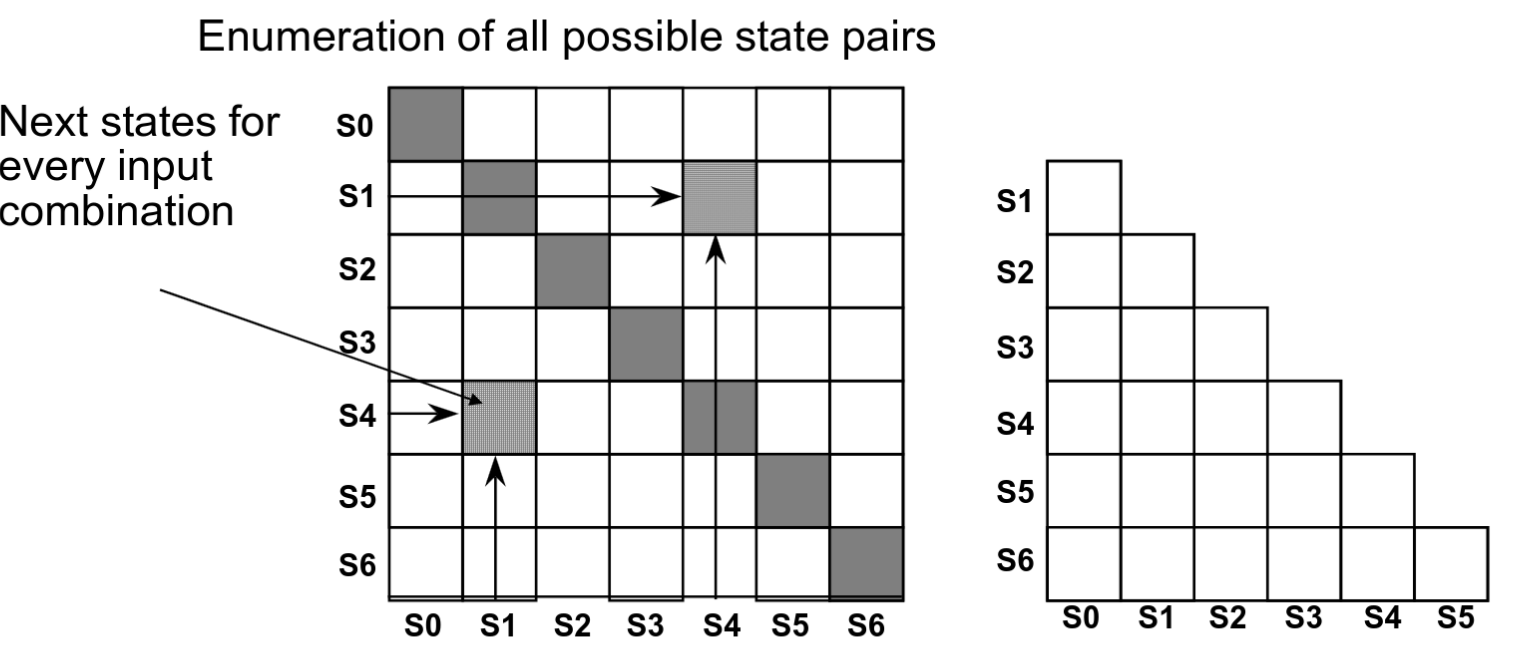
\includegraphics[scale=0.22]{../figures/implica.png}
\end{center}

An implication table is built by first enumerating all possible state pairs.
Then for each pair, we write the possible next states for every combination of state 1 and state 2.
We need this to determine which states can be combined.

Note that each entry $X_{ij}$ of the implication table will be equal (if not mirrored) to entry $X_{ji}$, so we can keep only the lower (or upper) diagonal.

Thus the pipeline:
\begin{itemize}
	\item After filling the table, with elements $X{ij}$: the row is $S_i$, the column is $S_j$;
	\item $S_i$ is equivalent to $S_j$ if the outputs are the same (first condition) and if the next states in the table are equivalent;
	\item $X_{ij}$ aids in this: it contains the next states of $S_i$ and $S_j$ that must be equivalent in order that $S_i$ and $S_j$ are equivalent;
	\item If $S_i$, $S_j$ have different outputs, delete $X_{ij}$, so that we don't accidentally flag false positives in the table (the first condition must be enforced elsewhere).
\end{itemize}

Some extra attention might be needed as we have to take into account the current simplifications as we move through the table.
To be clearer:
\begin{enumerate}
	\item Build the implication table with an element for each pair of states;
	\item Put "X" in the $S_i$, $S_j$ cell if outputs differ. Otherwise, write the implications for each input combination (first condition);
	\item Move in the table from the top and from the left. If the $S_i$, $S_j$ cell contains the $S_m$, $S_n$ pair and that pair contains “X”, put “X” also in $S_i$, $S_j$;
	\item Execute step 3 until no “X” are added;
	\item Each $S_i$, $S_j$ pair corresponding to a cell without “X” is equivalent.
\end{enumerate}

Note that what we are doing is not \textit{proving} states are equivalent, but finding if saying that two states are equivalent is a contradiction, which is looser and allows more options.

\subsection{State encoding}

\textbf{State encoding} entails assigning unique bit representation to each state.
Different encodings may reduce circuit size, or we might have a tradeoff between size and performance.

Types of encodings:
\begin{itemize}
	\item \textbf{Minimum-bitwidth binary} encoding: uses fewest bits via binary code;
	\item \textbf{One-hot} encoding: one high bit per status. A bit being ‘1’ corresponds to a particular state. This can give fewer gates and only one level of logic: we don't have to decode states, so we get less delay than two levels of logic (for decoding), meaning faster clock frequency;
	\item \textbf{Output} encoding: interestingly, we can have an encoding method where the state encoding is same as the output values. This is possible if enough outputs, all states with unique output values.
\end{itemize}

\subsection{Carry Look-Ahead}

Let's continue our study of optimization by looking at \textbf{CLA}, that is \textit{Carry Look-Ahead Adders}.

This is a form of \textit{datapath component optimization}: we can make some components faster (but bigger), or smaller (but slower), than the straightforward datapath components.

In this lesson we build a faster (but bigger) adder than the carry-ripple adder, knowing that we could also do this for the other datapath components.

We already built a normal \textit{carry-ripple adder}.
It functioned similar to adding by hand, column by column.
The problem is that it's \textit{slow}: the output is not correct until the carries have rippled to the left, which is a pretty long (and slow) critical path.

\par\smallskip

The idea is to modify the carry-ripple adder.
For a stage’s carry-in, don’t wait for carry to ripple, but rather directly compute from inputs of earlier stages.
This is called \textit{Look-Ahead} because the current stage "looks ahead" at previous stages rather than waiting for carry to ripple to current stage

\begin{center}
	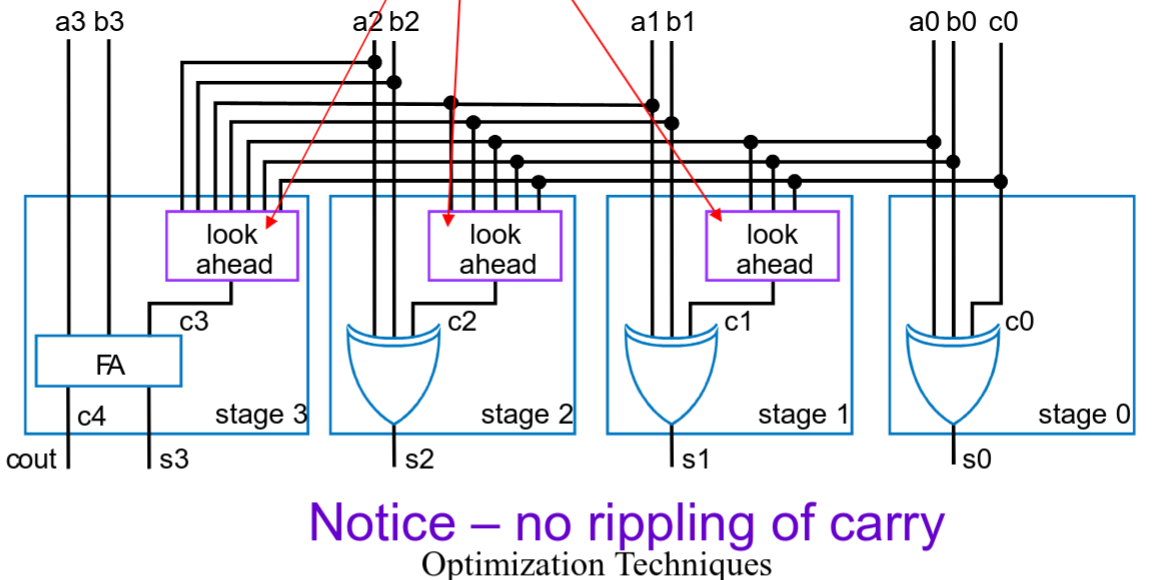
\includegraphics[scale=0.25]{../figures/dumb_cla.png}
\end{center}

Notice that this is quite unfeasible.
If we define the carry lookahead logic function as a function of external inputs, we solve the waiting for ripple problem, but equations get too big, which is not efficient.
We need a better form of lookahead circuit.

\par\smallskip

We can derive the lookahead formulas by examining the implementation of a given adder. We had established that the carry bit of a full adder computing $x+y$ is given by:

\[
C_i = G_i + P_i \cdot C_{in}
\]

where $G_i = x_i \cdot y_i$ and $P_i = x_i \oplus y_i$ are called the \textit{generate} and \textit{propagate} signals of the carry at bit $i$. Intuitively, these indicate whether a carry is generated or propagated at bit $i$, respectively.

We can then derive the expanded formulas by repeated substitution:

\[
C_0 = G_0 + P_0 \cdot C_{in}
\]

\[
C_1 = G_1 + P_1 \cdot G_0 + P_1 \cdot P_0 \cdot C_{in}
\]

\[
C_2 = G_2 + P_2 \cdot G_1 + P_2 \cdot P_1 \cdot G_0 + P_2 \cdot P_1 \cdot P_0 \cdot C_{in}
\]

\[
\begin{aligned}
C_3 ={}& G_3 + P_3 \cdot G_2 + P_3 \cdot P_2 \cdot G_1 \\
&+ P_3 \cdot P_2 \cdot P_1 \cdot G_0 \\
&+ P_3 \cdot P_2 \cdot P_1 \cdot P_0 \cdot C_{in}
\end{aligned}
\]

These carry signals are then fed directly to their respective full adders, which no longer need to wait for the carry to ripple through the preceding full adders.

The architecture is now quite simpler, to the point that we can actually implement it on 4 bits:
\begin{center}
	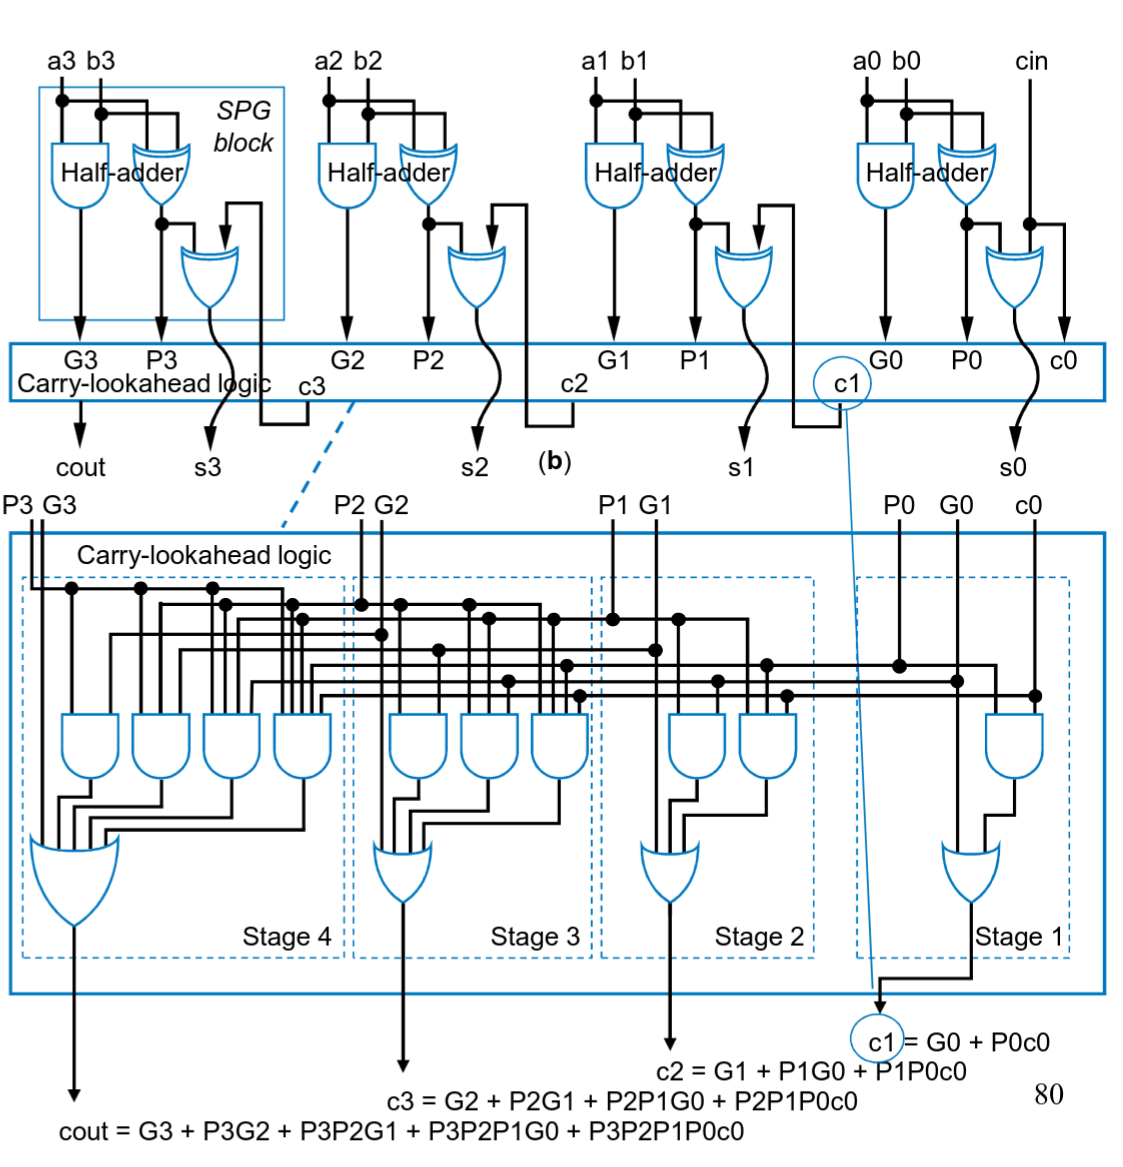
\includegraphics[scale=0.27]{../figures/good_cla.png}
\end{center}

\par\smallskip

We still have a problem gates get bigger in each stage.
The 4th stage has 5-input gates, the 32nd stage would have 33-input gates.
That is too many inputs for one gate, so it would require building from smaller gates, meaning more levels (slower), more gates (bigger).

One solution is to connect 4-bit CLA adders in carry-ripple manner, as we always did.
But we can do better by exploiting \textbf{hierarchy}.
Rather than rippling the carries, just repeat the carry-lookahead concept.
This requires a minor modification of the 4-bit CLA adder to add output $P$ and $G$.

\begin{center}
	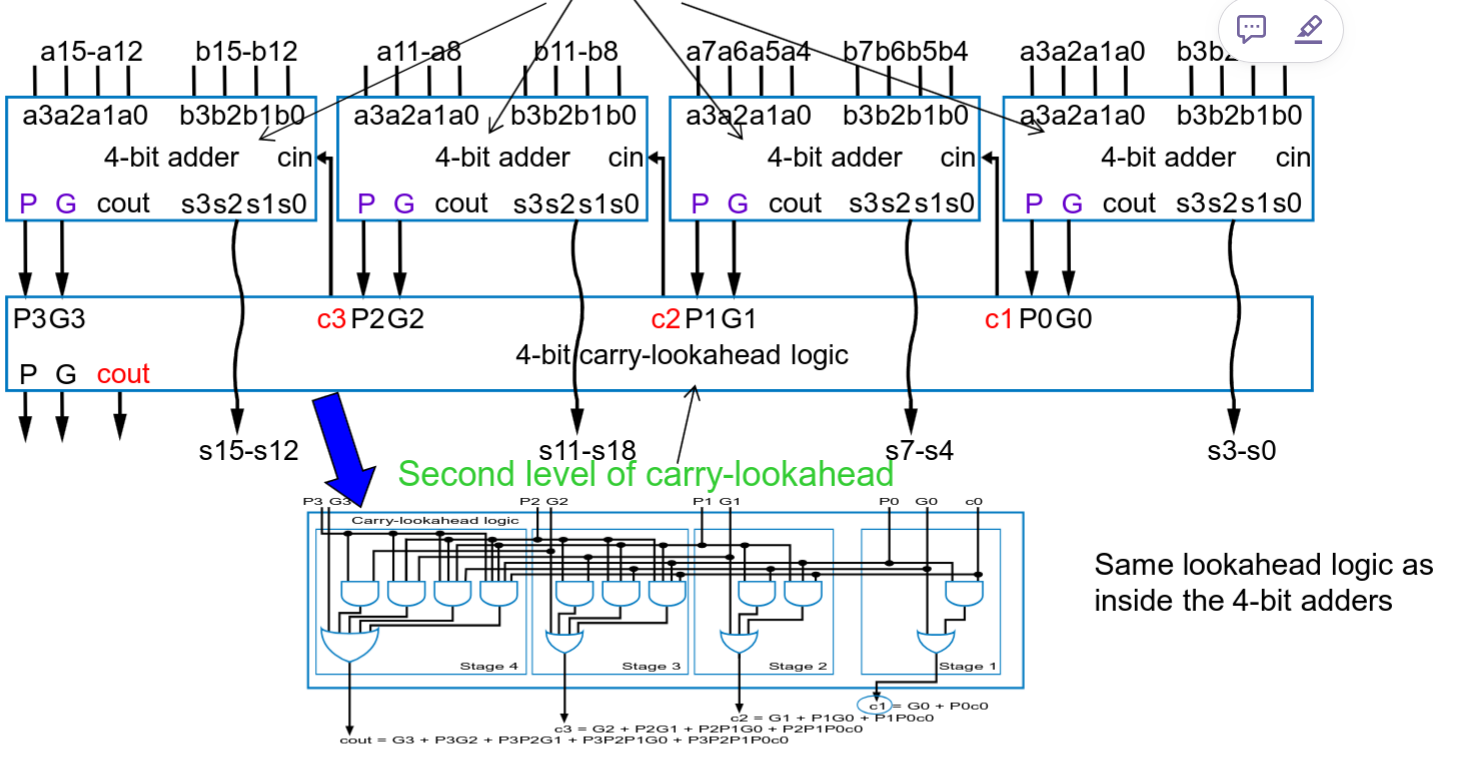
\includegraphics[scale=0.27]{../figures/great_cla.png}
\end{center}

\subsection{Validation and verification}

\textit{Simulation} is a tool to verify the \textit{correctness} of a system.
A \textit{formal method} is an application of Logic to the development of \textit{correct} systems.

These often play together.

\textbf{Correctness} itself is classically viewed as two separate problems:
\begin{itemize}
	\item \textbf{Validation}: are we building the right system?
	\item \textbf{Verification}: are we building the system right?
\end{itemize}

The difference between validation and verification shows the \textbf{limits} of verification (be it through simulation or formal verification).
Just because we have proved something correct does not mean
it will work! There are gaps where formal verification connects
with the real world.
Mainly: does the specification actually capture the designer's
intentions?

\subsubsection{Simulation}

For now we saw and used \textbf{simulation} as a verification tool.
Software Simulation is the application of simulation stimuli to a model of the intended circuit.
It's a traditional, basic, and flexible technique, applicable at any design level (physical, RTL, ...).

There are some difficulties in preparing "good" simulation patterns, as when the inputs grow in complexity it gets harder to cover corner cases.

Also, it is often impossible to simulate all input sequences to completely verify a design.

Other things we must consider:
\begin{itemize}
	\item On generation of input sequences:
we exercise a small fraction of system operations, based on manually developed patterns.
Patterns often biased towards anticipated sources of errors, but errors occur unexpectedly;

	\item On generation of expected outputs:
it is often difficult to compare outputs from different models and simulators

\end{itemize}

We might also encounter misunderstandings and inconsistencies due to increasing size of design team.

\par\smallskip

\textbf{Automated synthesis} might be an alternative to simulation and post-design verification, through the use of \textit{correct-by-construction} techniques.

\begin{itemize}
    \item Logic synthesis techniques have been successful in automating low-level (gate-level) logic design;
    \item Further progress is needed to automate the design process at higher levels of abstraction.
\end{itemize}

Until synthesis technology matures, high-level design must still be performed manually, which requires post-design verification.

\begin{itemize}
    \item The top-level specification and design must always be checked against the properties of the underlying idea;
    \item There is no golden reference at this level.
\end{itemize}

\subsubsection{Formal verification}

\textbf{Formal verification} appears as an alternative to all this.
It is the process of constructing a proof that a target system will behave in accordance with its specification.
This can be a complement to simulation to improve design quality.

We use mathematical reasoning to prove that an implementation satisfies a specification.
Like a mathematical proof: correctness of a formally verified hardware design holds regardless of input values.
It is complete, only with respect to a given property.

The consideration of \textit{all cases} is an implicit formal verification (proof by exhaustive verification).
It's a form of static analysis with no need for input/output sequences.

an generate an error trace if a property fails: helps us understand better, allows us to confirm by simulation.
Formal verification is often useful to detect and locate errors in designs.
What we want to do is prove the absence of bugs rather than their presence.

\par\smallskip

To prove the correctness of a design, both specification and implementation must be represented with mathematical models.
This is mathematical reasoning, equivalent to "all cases" simulations.

\begin{center}
	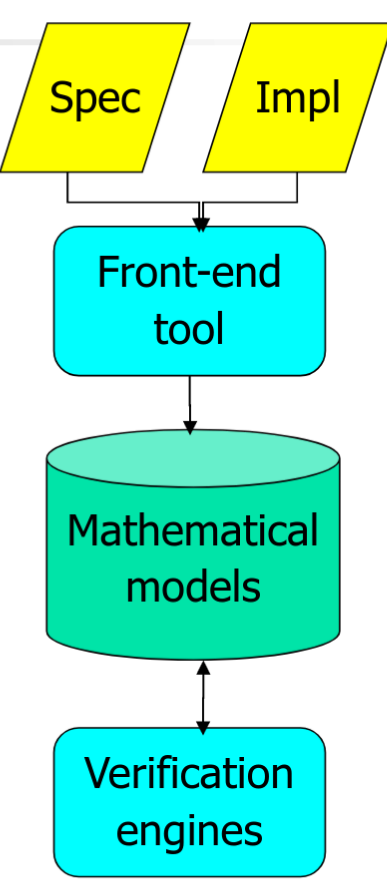
\includegraphics[scale=0.25]{../figures/fo_ver.png}
\end{center}

Possible mathematical models are:
\begin{itemize}
	\item \textit{Boolean functions} (which fall under \textbf{propositional logic}): how to represent and manipulate data on computers (bits of information);
	\item \textbf{First-order logic}: needed to represent "high level" designs where a concept of variables and quantifiers makes sense;
	\item \textbf{Higher-order logic}, such as \textit{theorem proving}: to us often an interactive (and computer assisted) method to prove conclusions based on a given property. 
\end{itemize}

\subsubsection{Simulation vs. Formal verification}

As a last note, the main point is not to have:
\begin{itemize}
	\item Correctness proofs of entire systems;
	\item Replacing simulation entirely.
\end{itemize}
but instead to:
\begin{itemize}
	\item Have one proof, which can replace many cases;
	\item Use formal methods in automatic input sequence generation.
\end{itemize}

To summarize:

\begin{itemize}
    \item \textbf{Simulation}:
    \begin{itemize}
        \item Complete (realistic) model;
        \item Partial verification.
    \end{itemize}

    \item \textbf{Verification}:
    \begin{itemize}
        \item Partial (abstract) model;
        \item Complete verification.
    \end{itemize}
\end{itemize}

\begin{itemize}
    \item Simulation is still needed to refine specifications, especially for large, complete designs.
    \item Verification can generate counterexamples (error traces), although false negatives are possible.
\end{itemize}

\subsubsection{Formal specification}

A \textit{specification} is a description of a system and its desired properties.
It's useful as a communication device:
\begin{itemize}
\item Between customer and designer;
\item Between designer and implementor;
\item Between implementors and tester.
\end{itemize}
It is a companion document to the system’s source code, but at a
higher level of abstraction
Properties relate to function, interfaces, timing, performance,
power, layout, etc...

A \textbf{formal specification} is the use of formal methods (a language with
mathematically-defined syntax and semantics) to describe the
intended behavior of the system.

The language of logic provides an unambiguous method of recording
the specification.

We can reason about a formal specification to check that the system
specified will possess other desired properties.

\par\smallskip

At this points other terms can be defined in function of specification:
\begin{itemize}
	\item \textbf{Formal validation}: Can we use logic to help ensuring that
the specification is complete, consistent, and accurately
captures the customer’s requirements?
	\item \textbf{Formal verification}: Can we use logic to help ensuring that
the system built faithfully implements its specification?
\end{itemize}

A method is said to be \textit{formal} if its rules for manipulation are based on
form (syntax) and not on contents ( semantics).

The Majority of existing formal techniques are based on some
flavor of formal (symbolic) logic: Propositional logic, Predicate
Logic, other logic.
The logic formalisms we use were already detailed above (in 9.3.2).

The \textbf{properties} we might want from a specification can be:
\begin{itemize}
	\item \textbf{Safety} properties: "undesirable things cannot happen";
	\item \textbf{Liveness} (progress) properties: desirable state repeatedly or eventually reached.
\end{itemize}

\subsubsection{Formal logic}

\textbf{Formal logic}: every logic comprises a formal language for making statements about
objects and reasoning about properties of these objects.
This is by definition formal.

Statements in a logic language are constructed according to a
predefined set of formation rules (depending on the language) called
syntax rules.
Statements that comply with the syntax are called well-formed
formulae.
A logic language can be used in different ways, through well-formed formulae.

\subsubsection{Model theory}

The second use of a logic language is for
expressing statements that receive a meaning
when given an interpretation.

The language of logic is used here to formalize
properties of structures, to determine when a
statement is true on a structure.

This use of a logic language is called
\textbf{model theory}.

It forces a
precise and
rigorous definition of the
concept of
truth on a structure.

\subsubsection{Interactive vs Automated methods}

2 main types of formal verification methods.

\begin{itemize}
	\item \textbf{Interactive} (deductive) methods:
\begin{itemize}
	\item 
Theorem Proving: relationship between a specification and an
implementation is a theorem in a logic, to be proven within the
context of a proof calculus.
\end{itemize}

	\item \textbf{Automated} methods:
		\begin{itemize}
			\item Combinational Equivalence Checking: proof of structural equivalence
of logic designs;
\item Sequential Equivalence Checking: proof of behavioral equivalence of
FSMs;
\item Model Checking: proof of (temporal) logic properties (safety \&
liveness) against a semantic model of the design;
\item Invariant Checking (safety property);
\item Language Containment (model checking of $\omega$-automata.
		\end{itemize}
\end{itemize}

\end{document}
